\documentclass{article}
\usepackage{graphicx} % Required for inserting images
\usepackage{amsmath}
\usepackage{amsfonts}
\usepackage{booktabs}

\title{24.12.17 Eligibility Check Benchmark}
\author{Xun Zhang \quad \quad Wuyun Siqin \quad \quad Bingsheng Zhang \\
Zhejiang University, CHN \\
22221024@zju.edu.cn \quad 3210101763@zju.edu.cn \quad bingsheng@zju.edu.cn}
\date{December 2024}

\begin{document}

\maketitle

\section{Circuit Implementation}

\subsection{Mapping and Merkle Tree}

We implemented the optimization in the paper:
\\
\\
\textit{Fortunately,
we don’t actually need to evaluate $\phi$ in the proof: we can replace stake in the tree with $\phi(stake)$ and proceed with the comparison directly}
\\
\\
So we replace the $stake$ by $\phi(stake)$ in our merkle tree construction.


And we use the mapping function in the Mithril open source code:

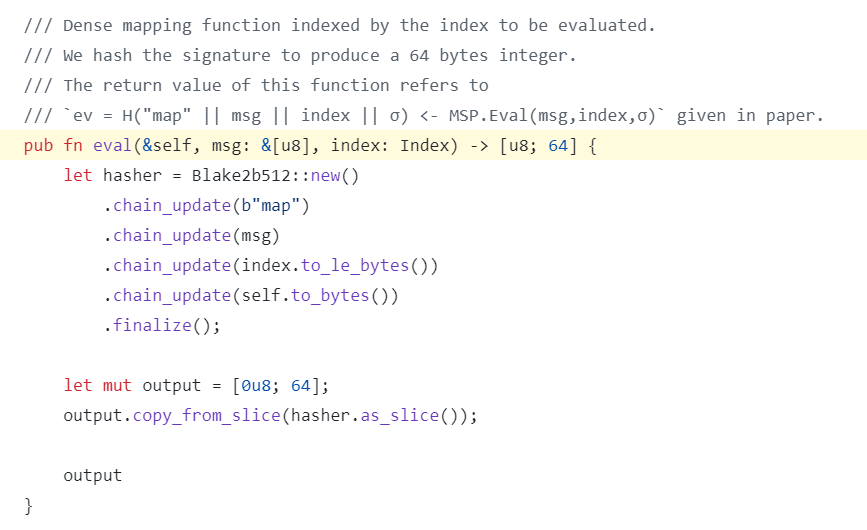
\includegraphics[width=1\linewidth]{mithril-mapping-code.png}


The corresponding description in the paper as following:
\\
\\
\textit{For the concatenation proof system PSC in Section 5.2 we use a random oracle
$H: \{0,1\}^* \rightarrow \mathbb{Z}_p $for the mapping as: $M_{mag,\mathsf{index}}^\sigma(\sigma)= H("map"||msg||\mathsf{index}||\sigma)$}
\\
\\
We instantiate the hash function as Poseidon function, which is same as the merkle tree.


\subsection{Comparison}

For the comparison between $\phi(stake)$ and mapping result, we use a compare gate in halo2-lib.

Note that in our circuit, the value of $\phi(stake)$ is a big integer in the prime filed, and we compare it with a hash ouput(also a big integer). This process is different from the Mithril code because they do not actually compute a $\phi(stake)$.

Below is our code implementation:


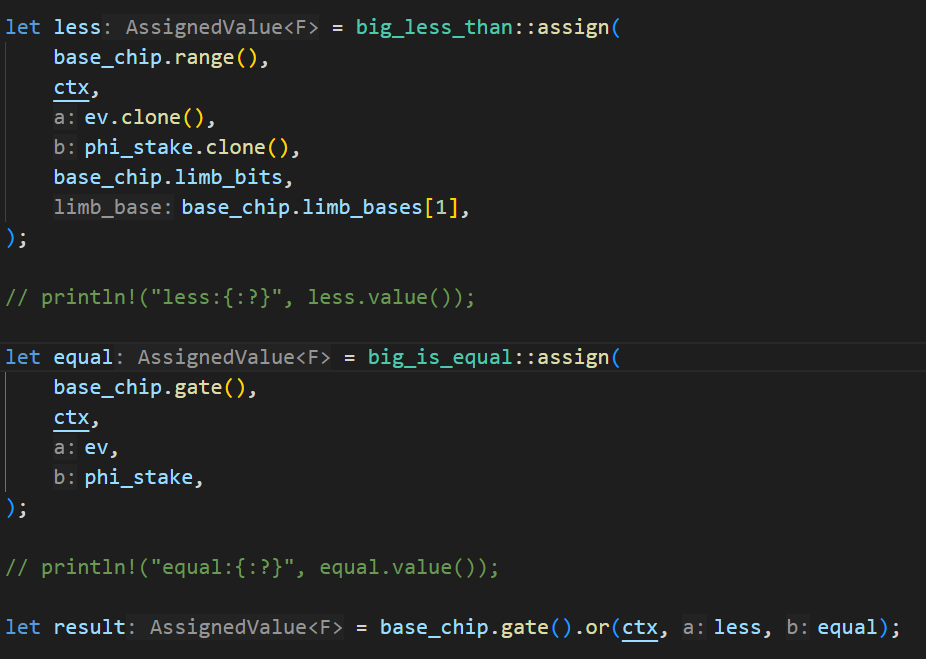
\includegraphics[width=1\linewidth]{compare_circuit_code.png}


Due to the complex implementation mechanism of halo2-lib's integer backend, this comparison circuit may have lower efficiency.


\section{Benchmark}

We benchmarked the performance of eligibility check circuit, including mapping function and comparison function. This is just a linear time task, see reults below:

\begin{table}[htbp]
    \centering
    \renewcommand{\arraystretch}{1.5} % 增加行间距
    \setlength{\tabcolsep}{10pt} % 增加列间距
    \begin{tabular}{cccccc} \toprule
        \textbf{num} & \textbf{128} & \textbf{256} & \textbf{512} & \textbf{1024} & \textbf{2048}  \\ \midrule
        Proving/s & 12.8556 & 16.3610 & 22.8908 & 36.4483 & 63.0147 \\ 
        proof/bit & 1344 & 1920 & 2848 & 4800 & 8832 \\ 
        verifying/ms & 7.2702 & 7.5913 & 6.9618 & 8.8133 & 10.3663 \\ \bottomrule
    \end{tabular}
    \caption{eligibility check benchmark}
    \label{tab:eligibility_check_benchmark}
\end{table}




\end{document}
